\def\i{\item}
\graphicspath{{../pictures/c5/}}
%\chapter{MỘT SỐ YẾU TỐ THỐNG KÊ VÀ XÁC SUẤT}
\newpage
\section{BIỂU ĐỒ VÀ CÁC DẠNG BIỂU ĐỒ}
\subsection{CÁC KIẾN THỨC CẦN NHỚ}
\subsubsection{Biểu đồ tranh}
\begin{enumerate}[--,leftmargin=*]
	\i Biểu đồ tranh sử dụng biểu tượng hoặc hình ảnh để thể hiện dữ liệu. Biểu đề tranh có tính trực quan. Trong biểu đồ tranh, một biểu tượng (hoặc hình ảnh) có thể thay thế cho một số đối tượng.
	\i Vẽ biểu đồ tranh:
	\begin{enumerate}[Bước 1.,leftmargin=*]
		\i Chuẩn bị:
		\begin{enumerate}[+,leftmargin=*]
			\i Chọn biểu tượng hoặc hình ảnh đại diện cho dữ liệu.
			\i Xác định mỗi biểu tượng (hình ảnh) thay thế cho bao nhiêu đối tượng.
		\end{enumerate} 
		\i Vẽ biểu đồ tranh
		-- Bao gồm 2 cột:
		\begin{enumerate}[+,leftmargin=*]
			\i Cột 1: Danh sách phân loại đối tượng thống kê.
			\i Cột 2: Vẽ các biểu tượng thay thế đủ số lượng các đối tượng.
		\end{enumerate}
	\end{enumerate}
\end{enumerate}
\subsubsection{Biểu đồ cột}
\begin{enumerate}[--,leftmargin=*]
	\i Biểu đồ cột sử dụng các cột có chiều rộng không đổi, cách đều nhau và có các chiều cao đại diện cho số liệu đã cho để biểu diễn dữ liệu.
	\i Vẽ biểu đồ cột:
	\begin{enumerate}[Bước 1.,leftmargin=*]
		\i Vẽ hai trục ngang và dọc vuông góc với nhau:
		\begin{enumerate}[+,leftmargin=*]
			\i Trục ngang: Ghi danh sách đối tượng thống kê.
			\i Trục dọc: Chọn khoảng chia thích hợp với dữ liệu và ghi số ở các vạch chia.
		\end{enumerate}
		\i Tại vị trí các đối tượng trên trục ngang, vẽ những cột hinnhf chữ nhật:
		\begin{enumerate}[+,leftmargin=*]
			\i Cách đều nhau.
			\i Có cùng chiều rộng
			\i Có chiều cao thể hiện số liệu của các đối tượng, tương ứng với khoảng chia trên trục dọc.
		\end{enumerate}
		\i Hoàn thiện biểu đồ:
		\begin{enumerate}[+,leftmargin=*]
			\i Ghi tên biểu đồ.
			\i Ghi tên các trục số ghi số liệu tương ứng trên mỗi cột (nếu cần).
		\end{enumerate}
	\end{enumerate}
\end{enumerate}
\subsubsection{Biểu đồ cột kép}
\begin{enumerate}[--,leftmargin=*]
	\i Để so sánh một cách trực quan từng cặp số liệu của hai bộ dữ liệu cùng loại, người ta ghép hai biểu đồ cột thành một biểu đồ cột kép.
	\i Vẽ biểu đồ cột kép: \\
	Cách vẽ biểu đồ cột kép tương tự như cách vẽ biểu đồ cột. Nhưng tại vị trí ghi mỗi đối tượng trên trục ngang, ta vẽ hai cột sát cạnh nhau thể hiện hai loại số liệu của đối tượng đó. Các cột thể hiện của cùng một bộ dữ liệu của các đối tượng thường được tô chung một màu để thuận tiện cho việc đọc biểu đồ.
\end{enumerate}
\subsection{THỰC HÀNH GIẢI TOÁN}
\begin{vd}
	Biểu đồ tranh sau đây biểu diễn số lượng học sinh lớp $8A$ sử dụng các phương tiện khác nhau để đi đến trường
	\begin{center}
		\renewcommand{\arraystretch}{1.4}
		\begin{tabular}{|l|l|}
			\hline
			Đi bộ	 &  
\includegraphics[scale=0.4]{hs}
\includegraphics[scale=0.4]{hs} \\
			\hline
			Xe đạp 	  &  
\includegraphics[scale=0.4]{hs}
\includegraphics[scale=0.4]{hs}
\includegraphics[scale=0.4]{hs}
\includegraphics[scale=0.4]{hs}
\includegraphics[scale=0.4]{hs}
\includegraphics[scale=0.4]{hs}
\includegraphics[scale=0.4]{hs}        \\
			\hline
			Xe ô tô (đưa đón học sinh)	&  
\includegraphics[scale=0.4]{hs}
\includegraphics[scale=0.4]{hs}
\includegraphics[scale=0.4]{hs}
\includegraphics[scale=0.4]{hs}    \\
			\hline
			Phương tiện khác &	
\includegraphics[scale=0.4]{hs}\\
			\hline
		\end{tabular}
	
	\vspace*{5pt}
	(Mỗi 
\includegraphics[scale=0.4]{hs} ứng với 3 học sinh)
	\end{center}
	\begin{enumerate}[a),leftmargin=*]
		\i Lớp $8A$ có tất cả bao nhiêu học sinh.
		\i Có bao nhiêu học sinh đến trường bằng xe đạp.
		\i Lập bảng thống kê biểu diễn số lượng học sinh sử dụng các phương tiện đến trường.
		\i Tính tỉ số phần trăm học sinh đi bộ đến trường (làm tròn kết quả đến hàng phần mười).
	\end{enumerate}
	\loigiai{
		\textbf{Tìm cách giải:}
		\begin{enumerate}[a),leftmargin=*]
			\i Trên biểu đồ có bao nhiêu biểu tượng 
\includegraphics[scale=0.4]{hs}, mỗi biểu tượng 
\includegraphics[scale=0.4]{hs}  ứng với bao nhiêu học sinh. Từ đó tính được số học sinh lớp $8A$.
			\i Xác định số biểu tượng của  ``Xe đạp", từ đó sẽ tính được số học sinh đến trường bằng xe đạp.
			\i Tính số học sinh đi bộ đến trường, số học sinh đi xe ô tô (đưa đón học sinh) và số học sinh đi bằng phương tiện khác đến trường; từ đó lập bảng thống kê.
			\i Tỉ số phần trăm học sinh đi bộ đến trường  = $\dfrac{\text{Số học sinh đi bộ đến trường}}{\text{Tổng số học sinh lớp 8A}} \cdot 100\%$
		\end{enumerate}
		\textbf{Trình bày lời giải:}
		\begin{enumerate}[a),leftmargin=*]
			\i Số học sinh của lớp 8A là:  (học sinh)
			\i Số học sinh đến trường bằng xe đạp là:  (học sinh)
			\i Số học sinh đi bộ đến trường là:  (học sinh)\\
			Số học sinh đi xe ô tô (đưa đón học sinh) đến trường là:  (học sinh)\\
			Số học sinh đi bằng phương tiện khác đến trường là:  (học sinh)
			Ta có bảng thống kê sau:\\
			\begin{tabular}{|l|c|c|c|c|}
				\hline
				Phương tiện&	Đi bộ&	Xe đạp&	Xe ô tô&	Phương tiện khác\\
				\hline
				Số lượng học sinh&	6&	21&	12&	3\\
				\hline
			\end{tabular}
			\i Tỉ số phần trăm học sinh đi bộ đến trường là: $\dfrac{6}{42}\cdot100\% = 14,3 \%$  (kết quả đã được làm tròn đến hàng phần mười)
		\end{enumerate}
	}
\end{vd}
\begin{vd}
	Biểu đồ cột sau đây biểu diễn số lượng vé bán được với các mức giá khác nhau của một buổi hòa nhạc
	\begin{figure}[H]
		\centering
		\vspace*{-5pt}
		\captionsetup{labelformat= empty, justification=centering}
		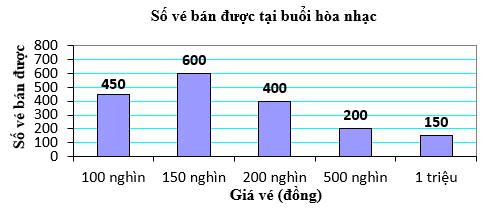
\includegraphics[width=0.5\linewidth]{1}
		\vspace*{-10pt}
	\end{figure}
	\begin{enumerate}[a),leftmargin=*]
		\i Tổng số vé bán được là bao nhiêu?
		\i Tổng số tiền bán vé thu được là bao nhiêu?
		\i Lập bảng thống kê biểu diễn số lượng vé bán được?
		\i Nếu nhà hát có 2500 ghế, thì số vé bán được chiếm bao nhiêu phần trăm?
	\end{enumerate}
	\loigiai{
		\begin{enumerate}[a),leftmargin=*]
			\i Tổng số vé bán được là: $450 + 600 + 400 + 200 + 150 = 1800$ (vé)
			\i Tổng số tiền bán vé thu được là: 
			\[450.100000 + 600.150000 + 400.200000 + 200.500000 + 150.1000000 = 465\,000\,000 \text{ (đồng).}\]
			\i Bảng thống kê
			\begin{center}
				\begin{tabular}{|l|c|}
					\hline
					Giá vé (đồng)&	Số vé bán được\\
					\hline
					100 nghìn&	450\\
					\hline
					150 nghìn&	600\\
					\hline
					200 nghìn&	400\\
					\hline
					500 nghìn&	200\\
					\hline
					1 triệu	&150\\
					\hline
				\end{tabular}
			\end{center}
			\i Nếu nhà hát có 2500 ghế, thì số vé bán được chiếm số phần trăm là:
			\[\dfrac{{1800}}{{2500}}.100\%  = 72\%\]
		\end{enumerate}
	}
\end{vd}
\begin{vd}
	Biểu đồ dưới đây biểu diễn số huy chương vàng và tổng số huy chương của các quốc gia tham dự Seagame lần thứ 30.
	\begin{figure}[H]
		\centering
		\vspace*{-5pt}
		\captionsetup{labelformat= empty, justification=centering}
		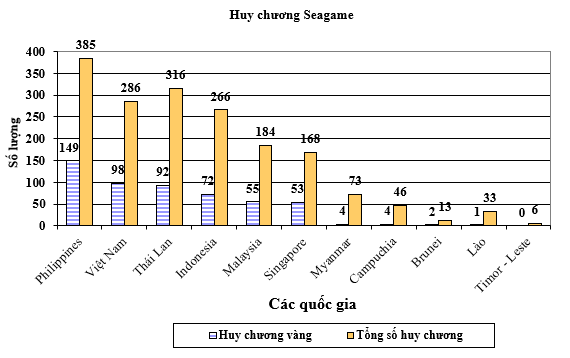
\includegraphics[width=0.5\linewidth]{2}
		\vspace*{-10pt}
	\end{figure}
	\begin{enumerate}[a),leftmargin=*]
		\i Kể tên 3 quốc gia có số huy chương vàng nhiều nhất?
		\i Sắp xếp các quốc gia theo thứ tự giảm dần về tổng số huy chương đạt được?
		\i Việc xếp hạng chung cuộc căn cứ trên số huy chương vàng, nếu hai quốc gia có số huy chương vàng bằng nhau thì quốc gia nào đạt được nhiều huy chương bạc hơn sẽ được xếp trên, trường hợp số huy chương bạc vẫn bằng nhau thì việc xếp hạng sẽ dựa trên số huy chương đồng đạt được. Theo em, Việt Nam xếp thứ mấy chung cuộc?
		\i Nếu xếp hạng theo tổng số huy chương đạt được thì Việt Nam đứng thứ mấy?
	\end{enumerate}
	\loigiai{
		\begin{enumerate}[a),leftmargin=*]
			\i Tên 3 quốc gia có số huy chương vàng nhiều nhất là: Philippines, Việt Nam, Thái Lan.
			\i Sắp xếp các quốc gia theo thứ tự giảm dần về tổng số huy chương đạt được là:
			Philippines, Thái Lan, Việt Nam, Indonesia, Malaysia, Singapore, Myanmar, Campuchia, Lào, Brunei, Timor – Leste.
			\i Việt Nam có số huy chương vàng chung cuộc đứng thứ hai sau Philippines nên chung cuộc Việt Nam đứng thứ hai.
			\i Nếu xếp hạng theo tổng số huy chương đạt được thì Việt Nam đứng thứ ba.
		\end{enumerate}
		\textbf{$^*$Nhận xét:} Đọc và phân tích dữ liệu từ các dạng biểu đồ
		\begin{enumerate}[--,leftmargin=*]
			\i \textbf{\textit{Biểu đồ tranh:}} Để đọc và mô tả dữ liệu ở dạng biểu đồ tranh, trước hết ta cần xác định một hình ảnh (một biểu tượng) thay thế cho bao nhiêu đối tượng. Từ số lượng hình ảnh (biểu tượng), ta sẽ có số đối tượng tương ứng. 
			\i \textbf{\textit{Biểu đồ cột:}} Khi đọc biểu đồ cột, ta nhìn theo một trục để đọc danh sách các đối tượng thống kê và nhìn theo trục còn lại để đọc số liệu thống kê tương ứng với các đối tượng đó (cần chú ý thang đo của trục số liệu khi đọc các số liệu).
			\i \textbf{\textit{Biểu đồ cột kép:}} Cũng tương tự như biểu đồ cột, nhưng lưu ý với mỗi đối tượng thống kế, ta thường đọc một cặp số liệu để tiện khi so sánh hơn, kém.
		\end{enumerate}
	}
\end{vd}
\begin{vd}
	Lớp $6A$ dự định tổ chức một trò chơi dân gian khi đi dã ngoại. Lớp trưởng yêu cầu cả lớp tham gia bình chọn cho 4 trò chơi được đề xuất (tất cả các bạn trong lớp đều tham gia bình chọn và mỗi bạn chỉ chọn một trò chơi). Sau khi thu phiếu, lớp trưởng tổng hợp và ghi lại kết quả như bảng sau:
	\begin{center}
		\begin{tabular}{|l|c|}
			\hline
			Trò chơi&	Số bạn chọn\\
			\hline
			Cướp cờ&	6\\
			\hline
			Nhảy bao bố&	15\\
			\hline
			Bịt mắt bắt dê&	9\\
			\hline
			Kéo co&	12\\
			\hline
		\end{tabular}
	\end{center}
	\begin{enumerate}[a),leftmargin=*]
		\i Hãy cho biết lớp 6A có bao nhiêu học sinh.
		\i Vẽ biểu đồ tranh biểu diễn bảng thống kê trên.
		\i Trò chơi nào được các bạn lựa chọn nhiều nhất.
	\end{enumerate}
	\loigiai{
		\textbf{Tìm cách giải:}
		\begin{enumerate}[a),leftmargin=*]
			\i Vì tất cả các bạn trong lớp đều tham gia bình chọn nên số học sinh của lớp 6A chính bằng tổng số bạn tham gia bình chọn.
			\i Hãy chọn số lượng tương ứng với 1 biểu tượng (có thể chọn 1 biểu tượng ứng với ước chung lớn nhất của các số liệu cho trong bảng)
			\i Quan sát biểu đồ tranh vừa vẽ thì trò chơi được bình chọn nhiều nhất là trò nào?
		\end{enumerate}
		\textbf{Trình bày lời giải}
		\begin{enumerate}[a),leftmargin=*]
			\i Lớp $6A$ có số học sinh là: $6 + 15 + 9 + 12 = 42$ (học sinh)
			\i Biểu đồ tranh biểu diễn bảng thống kê đã cho:
			\begin{center}
				\begin{tabular}{|c|c|}
					\hline
					Trò chơi	&Số bạn chọn\\
					\hline
					Cướp cờ &	$\heartsuit$$\heartsuit$\\
					\hline
					Nhảy bao bố& $\heartsuit$$\heartsuit$$\heartsuit$$\heartsuit$$\heartsuit$\\
					\hline
					Bịt mắt bắt dê&$\heartsuit$$\heartsuit$$\heartsuit$\\
					\hline
					Kéo co	&$\heartsuit$$\heartsuit$$\heartsuit$$\heartsuit$\\
					\hline
				\end{tabular}
			
			\vspace*{5pt}
			(Mỗi $\heartsuit$ ứng với 3 bạn chọn)
			\end{center}
			\i Trò chơi nhảy bao bố được các bạn lựa chọn nhiều nhất.
		\end{enumerate}
	}
\end{vd}
\begin{vd}
	Số lượt xem trên YouTube của một số nhóm nhạc tại các nước Đông Nam Á được cho trong bảng sau:
	\begin{center}
		\begin{tabular}{|l|c|c|c|c|}
			\hline
			Nhóm nhạc&	A&	B&	C&	D\\
			\hline
			Số lượt xem (triệu lượt)&	510&	1220&	960&	420\\
			\hline
		\end{tabular}
	\end{center}
	\begin{enumerate}[a),leftmargin=*]
		\i Vẽ biểu đồ cột biểu diễn bảng số liệu trên.
		\i Đơn vị tính số lượt xem của các các nhóm nhạc trong biểu đồ là gì?
		\i Hãy cho biết nhóm nhạc có lượt xem nhiều nhất là bao nhiêu lượt, nhóm có \i lượt xem ít nhất là bao nhiêu lượt?
	\end{enumerate}
	\loigiai{
		\begin{enumerate}[a),leftmargin=*]
			\i 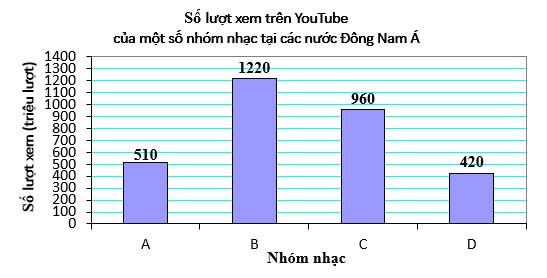
\includegraphics[width=0.5\linewidth]{3}
			
			\i Đơn vị tính số lượt xem của các các nhóm nhạc trong biểu đồ là triệu lượt.
			\i Nhóm nhạc có lượt xem nhiều nhất là nhóm B có 1220 triệu lượt xem, nhóm có lượt xem ít nhất là nhóm D có 420 triệu lượt xem.
		\end{enumerate}
	}
\end{vd}
\begin{vd}
	Thư viện trường THCS X đã ghi lại số lượng truyện tranh và sách tham khảo mà các bạn học sinh đã mượn vào các ngày trong tuần trong bảng sau:
	\begin{center}
		\begin{tabular}{|l|c|c|c|c|c|}
			\hline
			&Thứ hai&	Thứ ba&	Thứ tư&	Thứ năm&	Thứ sáu\\
			\hline
			Truyện tranh& 	25&	35&	20&	40&	30\\
			\hline
			Sách tham khảo&	15&	20&	30&	25&	20\\
			\hline
		\end{tabular}
	\end{center}
	\begin{enumerate}[a),leftmargin=*]
		\i Vẽ biểu đồ cột kép biểu diễn số lượng sách mà thư viện cho học sinh mượn?
		\i Tổng số truyện tranh mà các em học sinh đã mượn là bao nhiêu? 
		\i Loại sách nào được các em học sinh mượn nhiều hơn?
		\i Vào thời gian nào, sách tham khảo được mượn nhiều hơn truyện tranh?
	\end{enumerate}
	\loigiai{
		\begin{enumerate}[a),leftmargin=*]
			\i 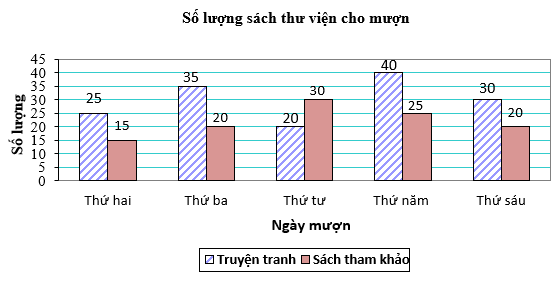
\includegraphics[width=0.5\linewidth]{4}
			\i Tổng số truyện tranh mà các em học sinh đã mượn là 
			\[25 + 35 + 20 + 40 + 30 = 150 \text{ (quyển)}\]
			\i Tổng số sách tham khảo mà các em học sinh đã mượn là 
			\[15 + 20 + 30 + 25 + 20 = 120 \text{ (quyển)}\]
			Loại sách mà các em mượn nhiều hơn là truyện tranh.
			\i Thứ tư là thời gian mà sách tham khảo mượn nhiều hơn truyện tranh.
		\end{enumerate}
	}
\end{vd}
\begin{vd}
	Bốn bạn Việt, Nam, Chiến, Thắng lần lượt sút bóng vào gôn. Mỗi bạn được đá  10 quả, mỗi lần đá vào gôn được 1 tích (), kết quả như sau
	\begin{center}
		\begin{tabular}{|l|l|}
			\hline
			Việt & \checkmark\checkmark\checkmark\checkmark\checkmark\\
			\hline
			Nam	& \checkmark\checkmark\checkmark\checkmark\checkmark\checkmark\checkmark\\
			\hline
			Chiến & \checkmark\checkmark\checkmark\checkmark\\
			\hline
			Thắng & \checkmark\checkmark\checkmark\checkmark\checkmark\checkmark\checkmark\checkmark\\
			\hline
		\end{tabular}
	\end{center}
	\begin{enumerate}[a),leftmargin=*]
		\i Hãy lập bảng thống kê số lần vào gôn của bốn bạn Việt, Nam, Chiến, Thắng  sau 10 lần đá.
		\i Vẽ biểu đồ cột biểu diễn bảng thống kê ở câu a? Bạn nào đá được vào gôn nhiều nhất sau 10 lần đá?
	\end{enumerate}
	\loigiai{
		\begin{enumerate}[a),leftmargin=*]
			\i \begin{tabular}{|l|c|}
				\hline
				&Số lần đá bóng vào gôn\\
				\hline
				Việt&	5\\
				\hline
				Nam	&7\\
				\hline
				Chiến&	4\\
				\hline
				Thắng&	8\\
				\hline
			\end{tabular}
			
			\i 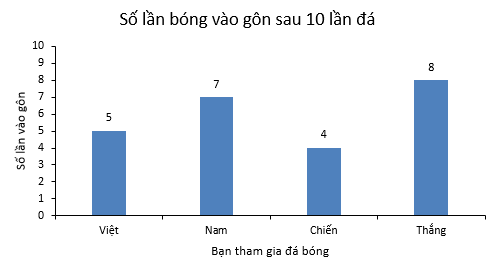
\includegraphics[width=0.5\linewidth]{5}
			
			Bạn Thắng đá bóng vào gôn được nhiều nhất sau 10 lần đá.
		\end{enumerate}
	}
\end{vd}
\begin{vd}
	Biểu đồ tranh trong hình thống kê số lượng táo bán được trong 4 tháng đầu năm 2021 của hai hệ thống siêu thị A và B.
%	Siêu thị A
%	
%	Tháng 1	 
%	Tháng 2	    
%	Tháng 3	   
%	Tháng 4	   
%	: 10 tấn     : 5 tấn
%	Siêu thị B
%	
%	Tháng 1	  
%	Tháng 2	    
%	Tháng 3	   
%	Tháng 4	    
%	: 10 tấn     : 5 tấn
	
	\begin{enumerate}[a),leftmargin=*]
		\i Hãy lập bảng thống kê số táo bán bán được trong 4 tháng đầu năm 2021 của hai hệ thống siêu thị A và B.
		\i Vẽ biểu đồ cột kép biểu diễn bảng thống kê ở câu a?
		\i Quan sát biểu đồ cột kép vừa vẽ và cho biết trong bốn tháng đầu năm, siêu thị nào bán được nhiều táo hơn.
	\end{enumerate}
	\loigiai{
		\begin{enumerate}[a),leftmargin=*]
			\i \begin{tabular}{|c|c|c|c|c|}
				\hline
				& Tháng 1	& Tháng 2&	Tháng 3	&Tháng 4\\
				\hline
				Siêu thị A&	10 tấn&	40 tấn&	25 tấn&	30 tấn\\
				\hline
				Siêu thị B&	15 tấn&	40 tấn&	25 tấn&	40 tấn\\
				\hline
			\end{tabular}
			\i 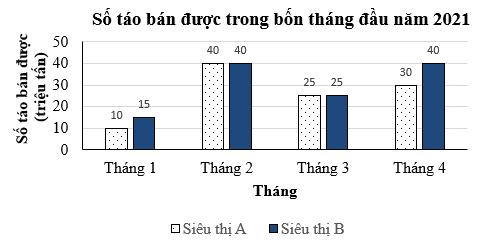
\includegraphics[width=0.5\linewidth]{6}
			\i Quan sát biểu đồ cột kép vừa vẽ thấy rằng trong bốn tháng đầu năm, siêu thị B bán được nhiều táo hơn.
		\end{enumerate}
		\textbf{$^*$Nhận xét:} 
		\begin{enumerate}[--,leftmargin=*]
			\i Dựa vào bảng thống kê, vẽ được biểu đồ tranh, biểu đồ cột (cột kép) tương ứng.
			\i Xử lý số liệu liên quan đến biểu đồ tranh để vẽ được biểu đồ cột
		\end{enumerate}
	}
\end{vd}
\subsection{MỞ RỘNG KIẾN THỨC}
\subsubsection*{Một số lỗi thường gặp khi vẽ biểu đồ cột}
Biểu đồ cột tuy là dạng rất đơn giản, dễ thực hiện nhưng vẫn có một số lỗi thường không chú ý. Đó là:
\begin{enumerate}[--,leftmargin=*]
	\i Ghi thiếu số liệu trên cột, thiếu đơn vị ở hai trục
	\i Đánh số đơn vị.
	\begin{enumerate}[+,leftmargin=*]
		\i Trên trục tung (chỉ số lượng) phải cách đều nhau và đầy đủ.
		\i Trên trục hoành nằm ngang (chỉ thời gian: năm, tháng,\ldots) tuy  không yêu cầu chính xác tuyệt đối như biểu đồ đồ thị nhưng phải đảm bảo tính tương đối hợp lí.
	\end{enumerate}
	\i Độ rộng các cột khác nhau.
	\i Cùng một đối tượng nhưng có kí hiệu khác nhau.
	\i Một số yếu tố phụ khác: thiếu tên biểu đồ hoặc bảng chú giải.
\end{enumerate}
$^*$Vẽ theo đúng trình trình tự bài cho, không được tự ý sắp xếp từ thấp tới cao hoặc ngược lại trừ khi bài có yêu  cầu sắp xếp lại.
\begin{figure}[H]
	\centering
	\vspace*{-5pt}
	\captionsetup{labelformat= empty, justification=centering}
	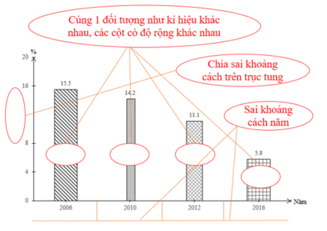
\includegraphics[width=0.5\linewidth]{7}
	\vspace*{-10pt}
\end{figure}
\subsection{BÀI TẬP TỰ LUYỆN} 
\subsubsection*{Mức cơ bản}
\Opensolutionfile{loigiaichung}[loigiaichuong40]
\begin{bt}
	Kết quả điều tra về màu áo đồng phục lớp được ưa thích nhất đối với một số bạn trong lớp được ghi lại như sau
	\begin{center}
		\begin{tabular}{|c|c|c|c|c|c|}
			\hline
			xanh lá	&hồng&	trắng&	tím&	đen&	vàng\\
			\hline
			vàng	&hồng&	hồng&	xanh lá&	tím	&trắng\\
			\hline
			hồng	&đen&	xanh lá&	vàng&	hồng&	tím\\
			\hline
			trắng	&vàng&	hồng&	xanh lá&	tím&	hồng\\
			\hline
			xanh lá	&tím&	hồng&	vàng&	hồng&	trắng\\
			\hline
		\end{tabular}
	\end{center}
	\begin{enumerate}[a),leftmargin=*]
		\i Lập bảng thống kê số lượng các bạn yêu thích mỗi màu áo đồng phục lớp.
		\i Vẽ biểu đồ cột biểu thị số lượng các bạn yêu thích mỗi màu áo đồng phục lớp.
	\end{enumerate}
	\begin{loigiaichuong40}
		\begin{enumerate}[a),leftmargin=*]
			\i Lập bảng thống kê số lượng các bạn yêu thích mỗi màu áo đồng phục lớp.
			\begin{center}
				\begin{tabular}{|c|c|c|c|c|c|c|}
					\hline
						Màu áo&	Xanh lá&	Hồng&	Trắng&	Tím&	Đen&	Vàng\\
						\hline
					Số học sinh& 5&9&4&5&2&5\\	 
					\hline
				\end{tabular}
			\end{center}
			\i Biểu đồ cột biểu thị số lượng các bạn yêu thích mỗi màu áo đồng phục lớp. 
			\begin{figure}[H]
				\centering
				\vspace*{-5pt}
				\captionsetup{labelformat= empty, justification=centering}
				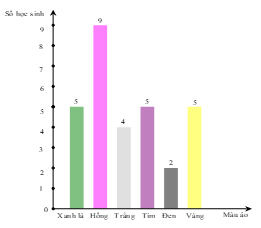
\includegraphics[width=0.5\linewidth]{9}
				\vspace*{-10pt}
			\end{figure}
		\end{enumerate}
	\end{loigiaichuong40}
\end{bt}
\begin{bt}
	Một cuộc khảo sát phương tiện đi làm trong toàn thể nhân viên của một công ty cho thấy có  35 nhân viên đi xe buýt, 5  nhân viên đi xe đạp,  20 nhân viên đi xe máy, 7  nhân viên đi ô tô cá nhân, không có nhân viên nào sử dụng các phương tiện khác. 
	\begin{enumerate}[a),leftmargin=*]
		\i Hãy lập bảng thống kê biểu diễn số lượng nhân viên sử dụng mỗi loại phương tiện đi làm.
		\i Vẽ biểu đồ cột biểu diễn số lượng nhân viên sử dụng mỗi loại phương tiện đi làm?
	\end{enumerate}
	\begin{loigiaichuong40}
		\begin{enumerate}[a),leftmargin=*]
			\i Bảng thống kê biểu diễn số lượng nhân viên sử dụng mỗi loại phương tiện đi làm.
			\begin{center}
				\begin{tabular}{|c|c|c|c|c|}
					\hline
					Loại phương tiện&	Xe buýt&	Xe đạp&	Xe máy&	Ô tô cá nhân\\
					\hline
					Số nhân viên& 35 &5&20&7\\
					\hline
				\end{tabular}
			\end{center}	 
			\i Biểu đồ cột biểu diễn số lượng nhân viên sử dụng mỗi loại phương tiện đi làm
			\begin{figure}[H]
				\centering
				\vspace*{-5pt}
				\captionsetup{labelformat= empty, justification=centering}
				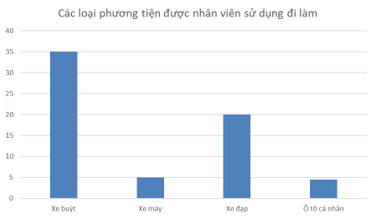
\includegraphics[width=0.5\linewidth]{10}
				\vspace*{-10pt}
			\end{figure}
		\end{enumerate}
	\end{loigiaichuong40}
\end{bt}
\begin{bt}
	Kết quả điều tra môn học yêu thích nhất của các bạn học sinh lớp $6C$ được cho bởi bảng sau:
	\begin{center}
		\begin{tabular}{|c|c|c|c|c|c|c|}
			\hline
			T&	V&	Đ&	NN&	Đ&	T&	V\\
			\hline
			V&	T&	V&	T&	NN&	V&	V\\
			\hline
			T&	T&	NN&	T&	V&	T&	NN\\
			\hline
			Đ&	NN&	T&	NN&	T&	NN&	T\\
			\hline
			NN&	T&	V&	T&	NN&	T&	T\\
			\hline
		\end{tabular}
		
		\vspace*{5pt}
		(Viết tắt: Đ: Địa lí; T: Toán; V: Văn; NN: Ngoại ngữ 1)
	\end{center}
	\begin{enumerate}[a),leftmargin=*]
		\i Bảng trên có tên là bảng gì? Hãy lập bảng thống kê tương ứng với dữ liệu cho ở bảng trên.
		\i Hãy vẽ biểu đồ cột biểu thị bảng thống kê vừa lập. Quan sát biểu dồ cho biết môn học nào được các bạn lớp $6C$ yêu thích nhất.
	\end{enumerate}
	\begin{loigiaichuong40}
		\begin{enumerate}[a),leftmargin=*]
			\i	Bảng trên có tên là bảng điều tra.\\
			Bảng thống kê:
			\begin{center}
				\begin{tabular}{|c|c|c|c|c|}
					\hline
					Tên môn học&	T&	Đ&	NN&	V\\
					\hline
					Số học sinh yêu thích&	15&	3&	9&	8\\
					\hline
				\end{tabular}
			\end{center}
			\i	Biểu đồ minh họa:
			\begin{figure}[H]
				\centering
				\vspace*{-5pt}
				\captionsetup{labelformat= empty, justification=centering}
				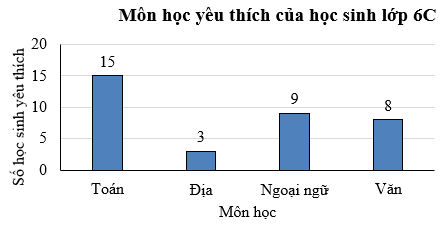
\includegraphics[width=0.5\linewidth]{11}
				\vspace*{-10pt}
			\end{figure}
			Qua biểu đồ trên ta thấy các bạn học sinh lớp $6C$ yêu thích nhất môn Toán.
		\end{enumerate}
	\end{loigiaichuong40}
\end{bt}
\begin{bt}
	Số học sinh khối 6 đến thư viện của trường mượn sách vào các ngày trong tuần được thống kê bảng sau:
	\begin{center}
		\begin{tabular}{|l|c|c|c|c|}
			\hline
			Ngày&	Thứ hai&	Thứ ba&	Thứ năm&	Thứ sáu\\
			\hline
			Số học sinh&	32	&16&	2&0	44\\
			\hline
		\end{tabular}
	\end{center}
	\begin{enumerate}[a),leftmargin=*]
		\i Vẽ biểu đồ tranh biểu diễn bảng thống kê trên?
		\i Học sinh đến thư viện vào ngày nào nhiều nhất, ngày nào ít nhất?
	\end{enumerate}
	\begin{loigiaichuong40}
		\begin{enumerate}[a),leftmargin=*]
			\i Ta có: ${\text{ƯCLN}}(32,16,20,44) = 4$\\
			Chọn mỗi biểu tượng  ứng với 4 học sinh mượn sách thư viện, ta có biểu đồ tranh sau
			\begin{center}
				\begin{tabular}{|l|l|}
					\hline
					Thứ hai&	\\
					\hline
					Thứ ba	&	\\
					\hline
					Thứ năm&	\\
					\hline 
					Thứ sáu	&	\\
					\hline
				\end{tabular}
			\end{center}
			\i Vào thứ sáu học sinh đến thư viện trường mượn sách đọc nhiều nhất, thứ ba học sinh mượn sách ít nhất.
			
		\end{enumerate}
	\end{loigiaichuong40}
\end{bt}
\begin{bt}
	Kết quả điều tra về loài hoa yêu thích của 30 bạn học sinh lớp 6A, bạn lớp trưởng thu được bảng dữ liệu như sau:
	\begin{center}
		\begin{tabular}{|c|c|c|c|c|c|}
			\hline
			H&	H&	M&	C&	C&	H\\
			\hline
			H&	Đ&	Đ&	C&	L&	H\\
			\hline
			H&	C&	C&	L&	C&	C\\
			\hline
			L&	M&	C&	Đ&	H&	C\\
			\hline
			C&	M&	L&	L&	H&	C\\
			\hline
		\end{tabular}
	
	\vspace*{5pt}
	(Viết tắt: H: Hoa Hồng; M: Hoa Mai; C: Hoa Cúc; Đ: Hoa Đào; L: Hoa Lan.)
	\end{center}
	\begin{enumerate}[a),leftmargin=*]
		\i Lập bảng thống kê số bạn học sinh lớp $6A$ yêu thích mỗi loại hoa. 
		\i Vẽ biểu đồ cột biểu diễn bảng thống kê vừa lập.
	\end{enumerate}
	\begin{loigiaichuong40}
		Thiếu
	\end{loigiaichuong40}
\end{bt}
\begin{bt}
	Hưởng ứng phong trào  ``Lá lành đùm lá rách" Liên đội trường THCS X phát động phong trào quyên góp vở ủng hộ các bạn học sinh miền núi. Số vở quyên góp trong hai đợt của các bạn đội viên các khối 6, 7, 8, 9 được thống kê trong bảng sau:
	\begin{center}
		\begin{tabular}{|c|c|c|c|c|}
			\hline
			&Khối 6&	Khối 7&	Khối 8&	Khối 9\\
			\hline
			Đợt 1&	180&	170&	200&	220\\
			\hline
			Đợt 2&	200&	180&	220&	190\\
			\hline
		\end{tabular}
	\end{center}
	\begin{enumerate}[a),leftmargin=*]
		\i Vẽ biểu đồ cột kép biểu diễn bảng thống kê ở trên.
		\i Theo em đợt quyên góp nào nhận được sự ủng hộ của các bạn nhiều hơn?
	\end{enumerate}
	\begin{loigiaichuong40}
		\begin{enumerate}[a),leftmargin=*]
			\i 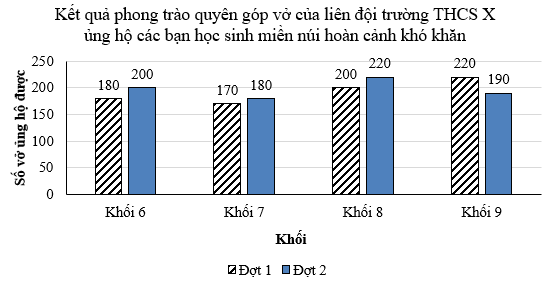
\includegraphics[width=0.5\linewidth]{12}
			\i Đợt 2 quyên góp nhận được sự ủng hộ của các bạn nhiều hơn.
		\end{enumerate}
	\end{loigiaichuong40}
\end{bt}
\subsubsection*{Mức nâng cao}
\begin{bt}
	Dương khảo sát về địa điểm làm bài tập ở nhà của các bạn học sinh lớp $6A$ bằng phiếu hỏi và thu được kết quả như sau:
	\begin{center}
		\begin{tabular}{|c|c|}
			\hline
			Địa điểm&	Số học sinh\\
			\hline
			Phòng khách& 6 \\
			\hline	 
			Phòng học	&  24 \\
			\hline
			Phòng ngủ	 & 9 \\
			\hline
			Địa điểm khác&	 3 \\
			\hline
		\end{tabular}
	\end{center}
	\begin{enumerate}[a),leftmargin=*]
		\i Chọn biểu đồ thích hợp và vẽ biểu đồ để biểu diễn số liệu này.
		\i Hãy cho biết lớp 6A có bao nhiêu học sinh. Theo em ở nhà các bạn học sinh lớp $6A$ hay làm bài tập ở đâu nhất?
	\end{enumerate}
	\begin{loigiaichuong40}
		\begin{enumerate}[a),leftmargin=*]
			\i Chọn biểu đồ cột và vẽ như sau:
			\begin{figure}[H]
				\centering
				\vspace*{-5pt}
				\captionsetup{labelformat= empty, justification=centering}
				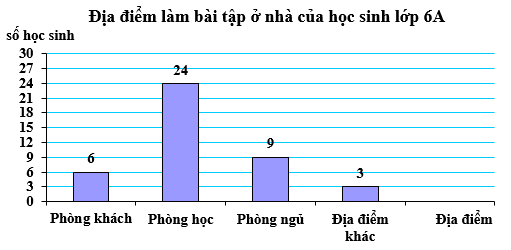
\includegraphics[width=0.5\linewidth]{13}
				\vspace*{-10pt}
			\end{figure}
			\i Lớp $6A$ có số học sinh là $6 + 24 + 9 + 3 = 42$  (học sinh).\\
			Theo em ở nhà các bạn học sinh lớp $6A$ hay làm bài tập ở phòng học nhất.
		\end{enumerate}
	\end{loigiaichuong40}
\end{bt}
\begin{bt}
	Biểu đồ tranh dưới đây cho biết lượng đồ chơi bán được tại cửa hàng của bố mẹ bạn An vào ngày Chủ nhật vừa qua. 
	\begin{center}
		\begin{tabular}{|l|l|}
			\hline
			Rubik& \\
			 \hline
			Ô tô điều khiển	& \\
			\hline
			Lego&	\\
			\hline
			Bộ đồ chơi cắt hoa quả&	\\
			\hline
			Pop It&	\\
			\hline
		\end{tabular}
	
	\vspace*{5pt}
	(Mỗi  ứng với ... số bộ đồ chơi được bán ra)
	\end{center}
	\begin{enumerate}[a),leftmargin=*]
		\i Biết rằng số bộ đồ chơi cắt hoa quả bố mẹ bạn An đã bán vào ngày chủ nhật đó là 6 bộ. Hãy điền vào dấu  ``\ldots" ở biểu đồ trên để chú thích cho mỗi biểu tượng .. ứng với bao nhiêu bộ đồ chơi đã được bán ra.
		\i Tổng số bộ đồ chơi mà cửa hàng đã bán được trong ngày chủ nhật vừa qua là bao nhiêu?
		\i Loại đồ chơi nào được bố mẹ An bán ra nhiều nhất trong ngày chủ nhật đó?
		\i Lập bảng thống kê số đồ chơi bán được trong ngày chủ nhật của cửa hàng.
	\end{enumerate}
	\begin{loigiaichuong40}
		\begin{enumerate}[a),leftmargin=*]
			\i Vì số bộ đồ chơi cắt hoa quả bố mẹ bạn An đã bán vào ngày chủ nhật đó là 6 bộ, trên biểu đồ ứng có 2 biểu tượng nên mỗi biểu tượng  ứng với 3 bộ đồ chơi đã bán được.
			\i Tổng số bộ đồ chơi đã bán trong ngày chủ nhật là: $\left( {5 + 3 + 3 + 2 + 8} \right).3 = 63$  (bộ)
			\i Đồ chơi Pop It được bố mẹ An bán ra nhiều nhất trong ngày chủ nhật.
			\i Bảng thống kê số đồ chơi bán được trong ngày chủ nhật của cửa hàng:
			\begin{center}
				\begin{tabular}{|l|c|}
					\hline
					&Số đồ chơi đã bán\\
					\hline
					Rubik&	15\\
					\hline
					Ô tô điều khiển&	9\\
					\hline
					Lego&	9\\
					\hline
					Bộ đồ chơi cắt hoa quả&	6\\
					\hline
					Pop It&	24\\
					\hline
				\end{tabular}
			\end{center}
		\end{enumerate}
	\end{loigiaichuong40}
\end{bt}
\begin{bt}
	Biểu đồ kép dưới đây biểu diễn số học sinh giỏi hai môn Toán và Ngữ văn của các lớp $6A$, $6B$, $6C$, $6D$ và $6E$
	\begin{figure}[H]
		\centering
		\vspace*{-5pt}
		\captionsetup{labelformat= empty, justification=centering}
		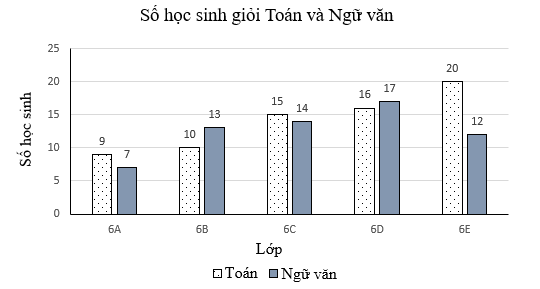
\includegraphics[width=0.5\linewidth]{8}
		\vspace*{-10pt}
	\end{figure}
	\begin{enumerate}[a),leftmargin=*]
		\i Số học sinh giỏi Toán của lớp nào nhiều nhất? ít nhất?
		\i Số học sinh giỏi Ngữ văn của lớp nào nhiều nhất? ít nhất?
		\i Số học sinh giỏi Toán của lớp $6E$ chiếm bao nhiêu phần trăm trong tổng số học sinh giỏi môn Toán của cả 5 lớp?
		\i Số học sinh giỏi Ngữ văn của lớp $6A$ chiếm bao nhiêu phần trăm trong tổng số học sinh giỏi môn Toán của cả 5 lớp?
		\i Bạn Nam nói lớp $6D$ có sĩ số là 34 học sinh. Theo em, bạn Nam nói đúng không? Vì sao?
	\end{enumerate}
	\begin{loigiaichuong40}
		\begin{enumerate}[a),leftmargin=*]
			\i Số học sinh giỏi Toán của lớp $6E$ nhiều nhất: có 20 bạn. Số học sinh giỏi Toán của lớp 6A ít nhất: 9 bạn
			\i Số học sinh giỏi Ngữ văn của lớp $6D$ nhiều nhất: có 17 bạn. Số học sinh giỏi Ngữ văn của lớp 6A ít nhất: 7 bạn.
			\i Số học sinh giỏi Toán của lớp $6E$ chiếm số phần trăm trong tổng số học sinh giỏi môn Toán của cả 5 lớp là
			\[\dfrac{{20}}{{9 + 10 + 15 + 16 + 20}}.100\%  = 28,6\%\]
			\i Số học sinh giỏi Ngữ văn của lớp $6A$ chiếm số phần trăm trong tổng số học sinh giỏi môn Toán của cả 5 lớp là
			\[\dfrac{7}{{7 + 13 + 14 + 17 + 12}}.100\%  = 11,11\%\]
			\i Bạn Nam nói lớp $6D$ có sĩ số là 34 học sinh có thể chưa đúng vì: trong lớp có thể có học sinh không giỏi môn Toán, môn Ngữ văn và có thể có học sinh giỏi cả 2 môn Toán và Ngữ văn.
		\end{enumerate}
	\end{loigiaichuong40}
\end{bt}
\begin{bt}
	Đài truyền hình Việt Nam muốn thăm dò ý kiến khán giả về thời lượng phát sóng phim truyện Việt Nam hàng tuần. Phiếu thăm dò đặt ra 4 mức: tăng thời lượng phát sóng, giữ như cũ, giảm, không ý kiến. Đài đã tiến hành thăm dò ba nhóm xã hội khác nhau: công nhân, nông dân, trí thức. Kết quả cuộc thăm dò như sau:
	\begin{center}
		\begin{tabular}{|l|c|c|c|}
			\hline
			&Công nhân&	Nông dân&	Trí thức\\
			\hline
			Tăng&	100&	300&	20\\
			\hline
			Như cũ&	200&	400&	30\\
			\hline
			Giảm&	50&	80&	5\\
			\hline
			Không ý kiến&	30	&70&	5\\
			\hline
		\end{tabular}
	\end{center}
	\begin{enumerate}[a),leftmargin=*]
		\i Nếu vẽ biểu đồ với bảng số liệu trên em có gặp khó khăn gì không?
		\i Nếu có thể em sẽ ghép cột hoặc dòng nào với nhau cho hợp lý để vẽ biểu đồ được dễ hơn. Hãy chọn biểu đồ thích hợp và vẽ biểu đồ để biểu diễn bảng số liệu vừa lập.
	\end{enumerate}
	\begin{loigiaichuong40}
		\begin{enumerate}[a),leftmargin=*]
			\i Số lượng trong bảng số liệu đã cho chênh lệch nhau rất lớn nên khi vẽ biểu đồ khá khó khăn.
			\i Vì tính chất các mức độ khác nhau, "không ý kiến" khác rất nhiều với việc  ``có bày tỏ ý kiến của mình" nên không thể ghép dòng với nhau. Hợp lý hơn ta có thể ghép cột  ``Trí thức" với cột "Công nhân" vì trí thức có vẻ gần với công nhân hơn nông dân (đều ở khu vực thành thị). Như vậy ta có bảng mới sau:
			\begin{center}
				\begin{tabular}{|l|c|c|}
					\hline
					&Công nhân và trí thức&	Nông dân\\
					\hline
					Tăng&	120&	300\\
					\hline
					Như cũ&	230&	400\\
					\hline
					Giảm&	55&	80\\
					\hline
					Không ý kiến&	34&	70\\
					\hline
				\end{tabular}
			\end{center}
		\end{enumerate}
		\begin{figure}[H]
			\centering
			\vspace*{-5pt}
			\captionsetup{labelformat= empty, justification=centering}
			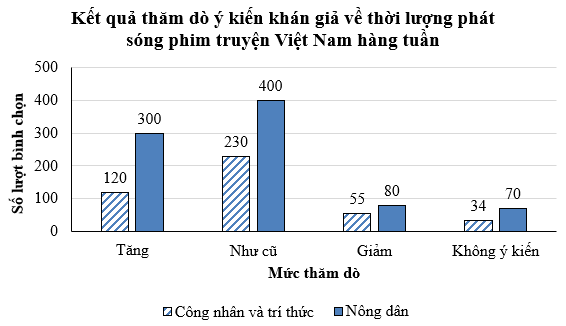
\includegraphics[width=0.5\linewidth]{14}
			\vspace*{-10pt}
		\end{figure}
	\end{loigiaichuong40}
\end{bt}
\Closesolutionfile{loigiaichung}